\begin{problem}[Munkres \S53, Ex.\,7(abcd)]
Let $G$ be a topological group with operation $\cdot$ and identity element
$x_0$. Let $\Omega(G,x_0)$ denote the set of all loops in $G$ based at
$x_0$. If $f,g\in\Omega(G,x_0)$, let us define a loop $f\otimes g$ by the
rule
\[
(f\otimes g)(s)=f(s)\cdot g(s).
\]
\begin{enumerate}[label=(\alph*)]
\item Show that this operation makes the set $\Omega(G,x_0)$ into a group.
\item Show that this operation induces a group operation $\otimes$ on
  $\pi_1(G,x_0)$.
\item Show that the two group operations $*$ and $\otimes$ on
  $\pi_1(G,x_0)$ are the same. [\emph{Hint:} Compute
  $(f*e_{x_0})\otimes(e_{x_0}*g)$.]
\item Show that $\pi_1(G,x_0)$ is Abelian.
\end{enumerate}
\end{problem}
\begin{proof}
For part (a) we need to show that the operation (i) $\otimes$ is
associtive, (ii) $\Omega(G,x_0)$ is closed under $\otimes$, (iii)
$\Omega(G,x_0)$ contains an identity element $e$ and (iv) for every
$f\in\Omega(G,x_0)$ there exists an element $f^{-1}$ such that $f\otimes
f^{-1}=f^{-1}\otimes f=e$. We shall proceed in order: (i) is easy since
the operation $\otimes$ is associative so for any triple
$f,g,h\in\Omega(G,x_0)$ we have
\[
(f\otimes g)\otimes h=(f(s)\cdot g(s))\otimes h=(f(s)\cdot g(s))\cdot h(s)
\]
which one clearly sees, by asociativity of $\cdot$, is the same as
$f\otimes(g\otimes h)$. (ii) Let $f,g\in\Omega(G,x_0)$ then, since $\cdot$
is continuous, the map $f\otimes g\colon I\to G$ is continuous and
\[
(f\otimes g)(0)=f(0)\cdot g(0)=x_0\cdot x_0=f(1)\cdot g(1)
=(f\otimes g)(1).
\]
Thus, $f\otimes g\in\Omega(G,x_0)$. Next, for (iii) consider the constant
loop $e_{x_0}(s)$. This map is clearly the identity on $\Omega(G,x_0)$ for
if $f\in\Omega(G,x_0)$ then $e_{x_0}\otimes f=e_{x_0}(s)\cdot f(s)=x_0\cdot
f(s)=f(s)$ for all $s$; similarly for $f\otimes e_{x_0}$. Lastly, (iv)
consider the map $f^{-1}(s)\coloneqq (f(s))^{-1}\colon I\to G$. This map is
continuous since taking the inverse in $G$ is continuous and composition of
continuous maps is continuous by Theorem 18.2(c). Lastly, note that
$f^{-1}(0)=x_0^{-1}=x_0$ similarly for $f^{-1}(1)$. Thus, $f^{-1}$ is a
loop and
\[
f^{-1}\otimes f=(f(s))^{-1}\cdot f(s)=x_0=f(s)\cdot(f(s))^{-1}=f\otimes f^{-1}
\]
so $\Omega(G,x_0)$ is closed under inverses. Thus, $\Omega(G,x_0)$ is a group.
\\\\
(b) The map $\otimes\colon\Omega(G,x_0)\times\Omega(G,x_0)\to\Omega(G,x_0)$
clearly induces a group operation on $\Pi_1(X,x_0)$ given by
$[f]\otimes[g]=[f\otimes g]$. All we need to check is that this operation
is in fact well defined on the equivalence class of loops based at $x_0$,
i.e., if $f_1\simeq_p f_2$ with path homotopy $H$ and $g_1\simeq_p g_2$
with path homotopy $K$ we want that $f_1\otimes g_1\simeq_p f_2\otimes
g_2$. But this is immediate via the homotopy $L(s,t)\coloneqq H(s,t)\cdot
K(s,t)\colon G\times I\to G$. This map is continuous since it can be
realized as the sequence of compositions
\[
(s,t)\longmapsto (H(s,t),K(s,t))\longmapsto H(s,t)\cdot H(s,t)
\]
where the intermediate step in the composition, i.e., the map from $I\times
I\to G\times G$, is continuous by Theorem 18.4 since $H$ and $K$ are
continuous and lastly $L(s,0)=H(s,0)\cdot K(s,0)=f_1(s)\cdot
g_1(s)=f_1\otimes g_1$ and $L(s,1)=H(s,1)\cdot K(s,1)=f_2(s)\cdot
g_2(s)=f_2\otimes g_2$. Thus, $f_1\otimes g_1\simeq_p f_2\otimes g_2$. It
follows that $\otimes$ is a well-defined binary operation on
$\pi_1(X,x_0)$.
\\\\
(c) Following the hint, we shall compute $(f*e_{x_0})\otimes(e_{x_0}*g)$.
Recall that
\[
f*e_{x_0}=
\begin{cases}
f(2s)&\text{for $s\in[0,1/2]$}\\
e_{x_0}(2s-1)&\text{for $s\in[1/2,1]$}
\end{cases}
\qquad\text{and}\qquad
e_{x_0}*g=
\begin{cases}
e_{x_0}(2s)&\text{for $s\in[0,1/2]$}\\
g(2s-1)&\text{for $s\in[1/2,1]$}
\end{cases}.
\]
Then
\begin{align*}
(f*e_{x_0})\otimes(e_{x_0}*g)
&=(f*e_{x_0})(s)\cdot (e_{x_0}*g)(s)\\
&=
\begin{cases}
f(2s)\cdot e_{x_0}(2s)&\text{for $s\in[0,1/2]$}\\
e_{x_0}(2s-1)\cdot g(2s-1)&\text{for $s\in[1/2,1]$}
\end{cases}\\
&=
\begin{cases}
f(2s)&\text{for $s\in[0,1/2]$}\\
g(2s-1)&\text{for $s\in[1/2,1]$}
\end{cases}\\
&=f*g.
\end{align*}
Since $f*e_{x_0}\simeq_p f$ and $e_{x_0}*g\simeq_p g$, we have at last that
\[
[f\otimes g]=[(f*e_{x_0})\otimes(e_{x_0}*g)]=[f*g].
\]
\\\\
(d) Lastly, we show that $\pi_1(X,x_0)$ must be Abelian. It suffices to
show that given a class of loop $[f]$ at $x_0$, the conjugacy class of
$[f]$ consists of the singleton $\{[f]\}$. First, note that if
$[g]\in\pi_1(X,x_0)$ then $[g^{-1}]\otimes [g]=[e_{x_0}]=[\bar g]*[g]$ so
$[g^{-1}]=[g^{-1}]\otimes ([g]*[\bar g])=[\bar g]$. Thus, we have
\begin{align*}
[\bar g]*[f]*[g]
&=\left([g^{-1}]*[f]\right)*[g*e_{x_0}]\\
&=\left([g^{-1}]*[f]\right)\otimes [g*e_{x_0}]\\
&=\begin{cases}
g^{-1}(2s)\cdot g(2s)&\text{for $s\in[0,1/2]$}\\
f(2s-1)\cdot e_{x_0}(2s-1)&\text{for $s\in[1/2,1]$}
\end{cases}\\
&=[e_{x_0}*f]\\
&=[f].
\end{align*}
It follows that $\pi_1(X,x_0)$ is Abelian.
\end{proof}
\newpage
\begin{problem}[(A)]
Prove Proposition F from the note on the Fundamental Group of the
Circle.
\end{problem}
\begin{proof}
Recall proposition F:
\begin{proposition*}[F]
\begin{enumerate}[label={\normalfont(\roman*)}]
\item $W$ takes the class of the path $f_n(s)=(\cos(2\pi ns),\sin(2\pi
  ns))$ to $n$ (and therefore $W$ is onto).
\item $W$ is one-to-one.
\item $W$ is a homomorphism.
\end{enumerate}
\end{proposition*}
(i) Now, recall that $W\colon\pi_1(S^1,x_0)\to\ZZ$ defined by
$W([f])\coloneqq w(f)$ where $w(f)=\tilde f(1)$ where $\tilde f\colon
I\to\RR$ is the lift of $f$, i.e. $p\circ \tilde f=f$. Now, let $f_n$ be a
path as above. Now, by Proposition C, since
\[
f_n(s)=(\cos(2\pi ns),\sin(2\pi ns))=(\cos(2\pi\tilde
f_n(s)),\sin(2\pi\tilde f_n(s)))
\]
and $\tilde f_n(0)=0=n\cdot 0$, by Proposition C, it follows that
$f_n(s)=ns$. Thus, $\tilde f(1)=n$.
\\\\
(ii) Let $f\colon I\to S^1$ be a loop at $x_0$. It suffices to show that if
$W([f])=n$ then $f\simeq_p f_n$. Let $\tilde f\colon I\to\RR$ be the lift
of $f$ and consider the path-homotopy $H\colon I\times I\to\RR$ defined by
$H(s,t)\coloneqq (1-t)\tilde f(s)+t(ns)$. This map is continuous by
Theorem 21.5 since it is multiplication from a topological space $I\times
I$ into $\RR$. Moreover, we have that
\begin{align*}
H(0,s)&=\tilde f(s)&H(1,s)&=ns
\end{align*}
and $H$ fixes the endpoints, i.e.,
\begin{align*}
H(t,0)&=(1-t)\cdot 0+t\cdot 0&
H(t,1)&=(1-t)n+tn\\
&=0&
&=n.
\end{align*}
At last, define the map $K\coloneqq p\circ H\colon I\times I\to S^1$. We
claim that this map is a path-homotopy from the class $f\simeq_p
f_n$. First, this map is continuous by Theorem 18.2(c) since it is a
composition of continuous maps. Secondly, we have that
\begin{align*}
K(0,s)&=p(H(0,s))&
K(1,s)&=p(H(0,s))\\
&=(\cos(2\pi\tilde f(s)),\sin(2\pi\tilde f(s)))&
&=(\cos(2\pi ns),\sin(2\pi ns))\\
&=f(s)&
&=f_n(s).
\end{align*}
and $K$ fixes the endpoints, i.e.,
\begin{align*}
K(t,0)&=p(H(t,0))&
K(t,1)&=p(H(t,1))\\
&=(\cos 0,\sin 0)&
&=(\cos 2\pi n,\sin 2\pi n)\\
&=x_0&
&=x_0.
\end{align*}
Thus, $f\simeq_p f_n$. It follows that if $W([f])=W([g])$ then $[f]=[g]$,
i.e., $W$ is one-to-one.
\\\\
(iii) Last but not least, we will show that $W$ is in fact a homomorphism
thus, proving that $W$ is an isomorphism $\pi_1(X,x_0)\cong\ZZ$. Let $f$
and $g$ be loops in $S^1$ at $x_0$ and let $\tilde f$ and $\tilde g$ be
their respective lifts to paths on $\RR$. Let $n\coloneqq W([f])$ and
$m\coloneqq W([g])$. Let $G\colon I\to\RR$ be the path $G(s)\coloneqq
n+\tilde g(s)$. Now, since $p(n+s)=p(s)$ for all $s\in\RR$, the path $G$ is
a lifting of $g$ begining at $n$. Thus, $\tilde f*G$ is defined, and
it is the lifting of $f*g$ that begins at $0$ and ends at $n+m$ so
\[
W([f]*[g])=n+m=W([f])+W([g]).
\]
Thus, $W$ is a homomorphism.
\end{proof}
\newpage
\begin{problem}[(B)]
Prove Lemma G from the note on the Fundamental Group of the Circle. (Hint:
one way to do this is to use the fact, which you don’t have to prove, that
if $\sim$ is the equivalence relation on $[a,a+1]$ which identifies $a$ and
$a+1$ then the restriction of $p$ induces a homeomorphism
$[a,a+1]/{\sim}\to S^1$.)
\end{problem}
\begin{proof}
Recall the statement of Lemma G:
\begin{lemma*}[G]
For each $a\in\RR$, the map
\[
p_a\colon(a,a+1)\longrightarrow S^1-\{p(a)\}
\]
given by $p_a(u)=p(u)$ is a homomorphism.
\end{lemma*}
We shall proceed by the hint. If $\sim$ is the equivalence
relation on $[a,a+1]$ which identifies $a$ and $a+1$ then the
restriction\footnote{\textcolor{Red}{What restriction? I'm not sure this
actually makes sense.}} of $p$ induces a homeomorphism $[a,a+1]/{\sim}\to
S^1$. Then, we claim that $[a,a+1]/{\sim}-\{[a]\}\approx(a,a+1)$ via the
restriction of $q\colon[a,a+1]\to[a,a+1]/{\sim}$ to $(a,a+1)$. Note that
$\left.q\right|_{(a,a+1)}$ is bijective: for every
$[x]\in[a,a+1]/{\sim}-\{[a]\}$, $x\in(a,a+1)$ so
$\left.q\right|_{(a,a+1)}(x)=[x]$ and if $[x]=[y]$ and $x\neq a$ or $a+1$
then $x=y$. Lastly, we show that $\left.q\right|_{(a,a+1)}$ is an open
map. By Lemma $C$, it suffices to prove this for basic open subsets of
$(a,a+1)$ so let us consider the open interval
$(b,c)\subset(a,a+1)$. Then
\[
\bigr(\left.q\right|_{(a,a+1)}\bigl)^{-1}\left(\left.q\right|_{(a,a+1)}((b,c))\right)
=\left\{\,x\in(a,a+1)\;\middle|\;\left.q\right|_{(a,a+1)}(x)\in\left.q\right|_{(a,a+1)}((b,c))\,\right\}
=(b,c)
\]
since $(b,c)$ is a saturated set, that is, it contains every
$\left.q\right|_{(a,a+1)}^{-1}([x])$ where
$[x]\in\left.q\right|_{(a,a+1)}(a,b)$ since the equivalence class of $x$
for $x\in(a,a+1)$ consists of the singleton $\{x\}$. It follows that
$(a,a+1)\approx[a,a+1]/{\sim}-\{[a]\}$ which, by Lemma A, is in turn
homeomorphic to $S^{-1}-\{\bar p([a])\}=S^{-1}-\{p(a)\}$.
\end{proof}
\newpage
\begin{problem}[(C)]
Show that for every point $x\in S^n$ the space $S^n-\{x\}$ is homeomorphic to
$\RR^n$. You may use the fact, shown in Step 1 of the proof of Theorem
59.3, that $S^n$ with the \emph{north pole} removed is homeomorphic to
$\RR^n$. (Hint: linear algebra.)
\end{problem}
\begin{proof}
By elementary linear algebra, extend the sets $\{x\}$ and
$\{(0,...,0,1)\}$ to orthonormal bases $\mathcal{B}_1$ and
$\mathcal{B}_2$ for $\RR^{n+1}$ (by Gram-Schmidt). Then, the
change of basis matrices from the strandard basis on $\RR^{n+1}$,
say $A_1$ and $A_2$ corresponding to $\mathcal{B}_1$ and
$\mathcal{B}_2$, respectively, are unitary linear
transformations. Then the composition $A\coloneqq
A_2A_1^{-1}\colon\RR^{n+1}\to\RR^{n+1}$ is a continuous map since
it is a bounded linear operator on $\RR^{n+1}$ with inverse
$A_1A_2^{-1}$ (which is also continuous since it is a bounded
linear operator on $\RR^{n+1}$) hence is a
homeomorphism. Moreover, since $A_1$ and $A_2$ are unitary then
$A_2A_1^{-1}=A$ is unitary, i.e., preserves the Euclidean
norm. It follows that the restriction
$\varphi\coloneqq\left.A\right|_{S^n}$ is a map from $S^1$ to $S^1$
is a homeomorphism by Lemma A with $\varphi(x)=(0,...,0,1)$. Now,
by Lemma A, the restriction
$\left.\varphi\right|_{S^n-\{x\}}\colon S^n-\{x\}\to
S^n-\{(0,...,0,1)\}$ is a homeomorphism. Thus, the composition
$\Phi\circ\bigl(\left.\varphi\right|_{S^1-\{x\}}\bigr)\colon
S^n-\{x\}\to\RR^n$, where $\Phi\colon S^n-\{(0,...,0,1)\}\to\RR^n$
is the stereographic projection from the north pole, gives a
homeomorphism from $S^n-\{x\}$ to $\RR^n$.
\end{proof}
\newpage
\begin{problem}[(D)]
Show that every loop in $S^n$ which is not onto is path-homotopic to a
constant path. (Hint: use Problem C).
\end{problem}
\begin{proof}
Fix $x_0\in S^n$ and let $f\colon I\to S^n$ be a loop at
$x_0$. If $f$ is not surjective, then there exists a point $x\in
S^{n}$ that does not get hit by $f$, i.e., $f(t)\neq x$ for all
$t\in I$. By Problem C, $S^n-\{x\}\approx\RR^n$ with
homeomorphism $\varphi$. Then $\varphi\circ f\colon I\to\RR^n$ is
a loop based at $\varphi(x_0)$. Since $\RR^n$ is
simply-connected, $\phi\circ f\simeq_p e_{\phi(x_0)}$ via the
homotopy $H$. Then $\varphi^{-1}\circ H\colon I\times I\to
S^n-\{x\}$ is a path homotopy from $f$ to $e_{x_0}$. Thus, if
$f\colon I\to S^n$ is not surjective, $[f]=[e_{x_0}]$.
\end{proof}
\newpage
\begin{problem}[(E)]
Let $X$ be a topological space and let $A\subset X$ be a deformation
retract. In the space $X/A$, the set $A$ is a point (because it is an
equivalence class). Show that this point is a deformation retract of
$X/A$. (Hint: use p.\,289 \# 9.)
\end{problem}
\begin{proof}
Let $H\colon X\times I\to X$ be a deformation retraction from $X$ to $A$,
that is, $H(0,x)=\id_X$ and $H(1,x)=r(x)$ where $r\colon X\to A$ is a
retraction of $X$ onto $A$ and $\iota\colon A\hookrightarrow X$ is
the inclusion of $A$ into $X$. Let $p\colon X\to X/A$ be a quotient
map. Now, we want to construct a deformation retraction $h\colon X/A\times
I\to X/A$ from the quotient $X/A$ to $*$, which we shall use to denote the
image of $A$ in $X/A$ under $p$, and what better candidate than the map
induced by $p\circ H\colon X\times I\to X/A$ on the quotient $X/A\times
I$ into $X/A$. Consider the map $(p,\id_I)\colon X\times I\to X/A\times
I$. This map is a quotient map by Problem 9.2 (Munkres \S46,
x.\,9). Moreover, the map $p\circ H$ preserves the equivalence relation on
$X/A\times I$ since for any two representatives $(x_1,t)$ and $(x_2,t)$ of
$[(x,t)]$ in $X/A\times I$, we have $H(x_1,t)=H(x_2,t)$ if $x\in X-A$ and
$H(x_1,t)=H_2(x_2,t)$ so $p(H(x_1,t))=p(H(x_2,t))$ and if $x_1,x_2\in
A$ then $H(x_1,t),H(x_2,t)\in A$ so $p(H(x_1,t))=p(H(x_2,t))$. Thus, by
Theorem Q.3 the map $h\colon X/A\times I\to X/A$ induced by $H$, i.e., the
map defined  by $h(x,t)\coloneqq[H(x,t)]$, is continuous and the diagram
\begin{center}
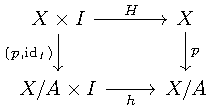
\includegraphics{figures/hw-11-def-retract}
\end{center}
commutes. We claim that $h$ is a deformation retraction from $X/A$ to
$*$. To that end, it suffices to show that $h(x,0)=\id_{X/A}$ and, using
suggestive notation, $h(x,1)=\bar r$ where $\bar r\colon X/A\to *$ is a
retraction of $X/A$ onto $A$ and $\bar\iota\colon *\hookrightarrow X/A$ is
the inclusion of $*$ into $X/A$. The first is easy to verify since
$h(x,0)=[H(x,0)]=[x]=\id_{X/A}$. Next, $h(x,1)=[H(x,1)]=[r(x)]$ and we
claim that $\bar r(x)\coloneqq [r(x)]$ is a retraction of $X/A$ into
$*$. The map $\bar r$ is continuous since $h$ is continuous (by Lemma 1
from Hw.\,\#9 Munkres \S18, Ex.\,11) and $\bar r\colon X/A\to *$ since
$r(x)\in A$ for every $x\in X$. It follows that $*$ is a deformation
retract of $X/A$.
\end{proof}

%%% Local Variables:
%%% mode: latex
%%% TeX-master: "../MA571-HW-Current"
%%% End:
